\subsection[Viterbi algorithm]{Uncovering Hidden states: Viterbi algorithm}
\label{sec:viterbi}

\begin{frame}
  \frametitle{Solve the best explanation problem}
  \begin{itemize}
  \item How can we answer the \emph{best explanation} problem?  \pause
  \item \textbf{Individually} most likely states
    \begin{equation}
      \label{eq:individually}
      \gamma_{t,i}=P(q_t = s_i \vert O, \lambda)
    \end{equation}
    \pause
  \item Computation
    \begin{equation}
      \label{eq:gamma_formula}
      \gamma_{t,i}=\frac{\alpha_{t,i}\beta_{t,i}}{P(O\vert \lambda)} =
      \frac{\alpha_{t,i}\beta_{t,i}}{\displaystyle\sum_{k=1}^{N}\alpha_{t,k}\beta_{t,k}}
    \end{equation}
    \pause
  \item Problems?
  \end{itemize}
\end{frame}

\begin{frame}
  \frametitle{Better optimality criterion}
  \begin{itemize}
  \item Can we find a better optimality criterion?  \pause
  \item Single best path \\
    $Q_{\text{best}} = [\hat{q}_1 \hat{q}_2 \cdots \hat{q}_T]$
    \begin{equation}
      Q_{\text{best}} = \underset{Q}{\operatorname{argmax}}\;
      P(Q \vert O, \lambda)
      = \underset{Q}{\operatorname{argmax}}\; P(Q, O \vert \lambda)
      \tag{\ref{eq:best-explanation}}
    \end{equation}
  \item \textbf{Viterbi algorithm} - dynamic programming
  \end{itemize}
\end{frame}

\begin{frame}
  \frametitle{$\delta$ variables}
  \begin{itemize}
  \item Introducing $\delta$ variables:
    \begin{equation}
      \label{eq:delta-definition}
      \delta_{t,i}=\underset{q_1,\ldots,q_{t-1}}{max} 
      P([q_1 q_2 \ldots q_{t-1} s_i], [o_1, o_2, \ldots o_t] \vert \lambda)
    \end{equation}
  \end{itemize}
  \begin{columns}
    \column{0.5\textwidth}
    \begin{itemize}
    \item $\delta_{t,i}$ - the highest probability for a sequence of
      $t$ states that ends in $s_i$ which accounts for the first $t$
      observations \visible<2>{
      \item the relation between \emph{sequential} $\delta$ variables:
        \begin{equation}
          \label{eq:delta-recurrence}
          \delta_{t,j} = [\underset{i}{max}\; \delta_{t-1,i} \cdot a_{i,j}] \cdot b_{j}(o_{t})
        \end{equation}}
    \end{itemize}
    \column{0.5\textwidth} \visible<2>{
      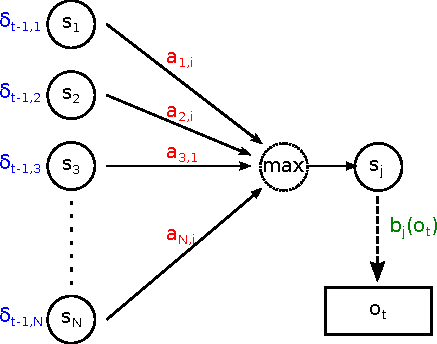
\includegraphics[width=\textwidth]{graphics/viterbi_path.pdf}
    }
  \end{columns}
\end{frame}

\begin{frame}
  \frametitle{Viterbi algorithm (I)}
  \begin{description}
  \item[1] Initialization: \\
    \begin{equation}
      \label{eq:viterbi-initialization}
      \begin{split}
        \delta_{1,i} & = \pi_{i}b_i(o_1), \quad 1 \le i \le N \\
        \psi_{1,i} & = 0
      \end{split}
    \end{equation}
  \item[2] Recursion: \\
    \begin{equation}
      \label{eq:viterbi-recursion}
      \begin{split}
        \delta_{t,j} & = [\underset{i }{max}\; \delta_{t-1,i} \cdot
        a_{i,j}] \cdot b_{j}(o_{t})
        \quad \scriptstyle{2 \le t \le T, 1 \le j \le N} \\
        \psi_{t,i} & = \underset{i}{argmax}\; \delta{t-1,i}\cdot
        a_{i,j} \quad \scriptstyle{2 \le t \le T, 1 \le j \le N}
      \end{split}
    \end{equation}
  \end{description}
\end{frame}

\begin{frame}
  \frametitle{Viterbi algorithm (II)}
  \begin{description}
  \item[3] Termination: \\
    \begin{equation}
      \label{eq:viterbi-termination}
      \begin{split}
        P(Q_{\text{best}} \vert O, \lambda) & = \underset{i}{max}\; \delta_{T,i} \\
        \hat{q}_T & = \underset{i}{argmax}\; \delta_{T,i}
      \end{split}
    \end{equation}
  \item[4] Backtracking: \\
    \begin{equation}
      \label{eq:viterbi-backtracking}
      \hat{q}_t = \psi_{t+1}(\hat{q}_{t+1}), \quad \scriptstyle{t=T-1,T-2,\cdots, 1}
    \end{equation}
  \end{description}
\end{frame}

